
\section{Design}

\subsection{Architettura del sistema}

\begin{figure}
    \centering
    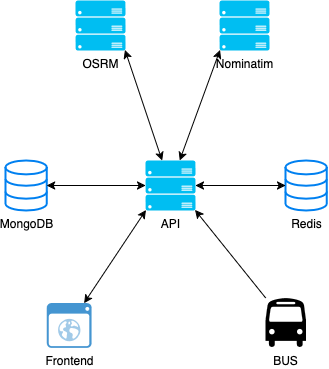
\includegraphics[width=0.6\linewidth]{images/architecture_diagram.png}
    \caption{Architettura del sistema}
    \label{fig:architecture-diagram}
\end{figure}

Data la complessità del progetto, il sistema è composto da numerosi componenti che interagiscono tra loro; in figura \ref{fig:architecture-diagram} è rappresentato un diagramma che descrive quali sono questi componenti e come comunicano tra loro.

\subsubsection{MongoDB e Redis}

MongoDB e Redis sono i due database utilizzati per memorizzare i dati del sistema.
Redis contiene al suo interno i dati in tempo reale di ciascun autobus che includono posizione, tempo di arrivo alla fermata successiva, i minuti di ritardo e le informazioni sulla fermata successiva. Di seguito è riportato un esempio del formato di questi dati:
\begin{lstlisting}[language=json]
{
    "position": [12.055590668167374,44.22314450204817],
    "minutesLate": 10,
    "timeToNextStop": 75.7,
    "nextStop": {
        "stopId": "6857d15047831cdd3f8550c4",
        "name": "Galilei"
    }
}
\end{lstlisting}

MongoDB invece contiene al suo interno tutti gli altri dati del sistema; questi dati includono:
\begin{itemize}
    \item informazioni sugli utenti
    \item informazioni su linee e fermate
    \item grafo del sistema di trasporto pubblico
    \item informazioni sulle corse
    \item tracce GPS dei percorsi delle linee
\end{itemize}

In figura \ref{fig:database-schema} è possibile vedere parte dello schema del database (è stata omessa la collezione contenente le informazioni degli utenti per semplificazione).

\paragraph{Bus Lines} La collezione \verb|bus_lines| contiene tutte le informazioni sulle linee; queste informazioni, oltre al nome della linea, includono i dati su ciascuna direzione della linea e la tabella degli orari.
Ciascuna direzione è a sua volta caratterizzata da nome, fermate e riferimenti alla traccia GPS del percorso; ciascuna fermata è un oggetto contenente l'id della fermata (che fa riferimento alla collezione \verb|bus_stops|), il nome della fermata (ridondato in modo da ridurre il numero di query da eseguire), il tempo necessario per arrivare alla fermata successiva e il riferimento alla traccia GPS che determina il percorso tra la fermata e quella successiva.
Come si può notare, tutte le tracce GPS sono memorizzate in una collezione separata dalle altre; è stata presa questa decisione per mantenere contenute le dimensioni dei documenti delle altre collezioni dato che queste tracce possono essere composte da molti punti e quindi occupare molto spazio.

\paragraph{Bus Stops} La collezione \verb|bus_stops| contiene tutte le informazioni riguardanti le fermate; queste informazioni includono nome, posizione della fermata e lista delle direzioni che passano per la fermata.
La lista delle direzioni è un array contenente il riferimento all'id della direzione (il campo \verb|directions._id| di \verb|bus_lines|); questo array è utile per ottenere in modo rapido la lista degli autobus che partono da una determinata fermata senza dover scansionare tutta la collezione \verb|bus_lines|,

\paragraph{Bus Rides} La collezione \verb|bus_rides| contiene tutte le informazioni riguardanti le corse degli autobus. Ciascun documento rappresenta una singola corsa in un determinato giorno e ad un determinato orario. Le corse sono caratterizzate da: riferimento alla linea e alla direzione (campi \verb|lineId| e \verb|directionId|), orario di partenza previsto, stato della corsa, lista (se è attiva o è terminata) e lista delle fermate.
La lista delle fermate è un array di oggetti contenenti id della fermata, nome, l'orario di arrivo previsto e un flag che indica se il bus è già passato da quella fermata oppure no.

\paragraph{Stops Connections} La collezione \verb|stops_connections| contiene le informazioni riguardanti le connessioni tra le fermate; ciascun documento si può considerare come un arco del grafo della rete di trasporto in cui ogni fermata è un nodo. Ogni arco è caratterizzato dai riferimenti alle fermate di partenza e arrivo (rispettivamente i campi \verb|from| e \verb|to|) e dalla lista delle linee che coprono il tragitto tra le due fermate; la lista delle linee (campo \verb|lines|) è un array di oggetti contenenti id della linea, id della direzione e tempo di percorrenza.

\paragraph{Routes} come accennato in precedenza la collezione \verb|routes| contiene le tracce GPS dei percorsi delle linee. Ciascun documento è caratterizzato da: id della direzione, tipo di traccia e la traccia vera e propria (il campo \verb|path|); il tipo indica se la traccia è parziale (ovvero il percorso tra due fermate) oppure completa (ovvero la traccia di tutta la linea).
Il campo \verb|path| è un array di oggetti ciascuno dei quali indica uno step della traccia; questi step sono caratterizzati da tempo di percorrenza e un array di geometrie spaziali in formato GeoJSON (campo \verb|path.geometry|).

\begin{figure}[H]
    \centering
    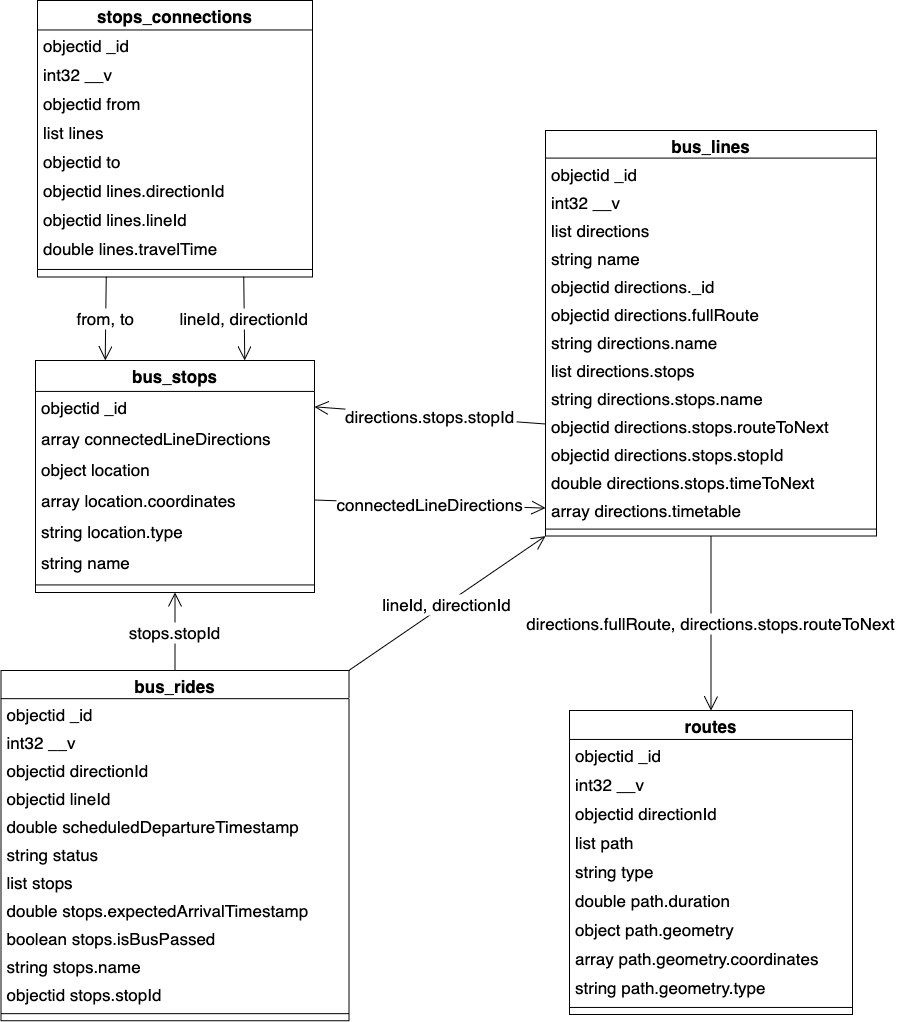
\includegraphics[width=1\linewidth]{images/database_schema.png}
    \caption{Schema del database}
    \label{fig:database-schema}
\end{figure}


\subsubsection{API}

Le API sono il componente che gestisce la logica del sistema e fa da ponte tra i client e le basi di dati e servizi esterni.
Sono state progettate e sviluppate seguendo il paradigma REST in modo da aderire a un modello standard e contemporaneamente avere un'architettura semplice e flessibile e tutti gli endpoint sono stati documentati utilizzando lo standard OpenAPI.
All'interno del repository è possibile trovare sia il file con le specifiche (\verb|api/api-schema.yaml|) che un file HTML contenente la documentazione generata in automatico (\verb|api/docs/index.html|); è possibile inoltre visualizzare la documentazione a \href{https://htmlpreview.github.io/?https://raw.githubusercontent.com/bambinim/CityBus/refs/heads/main/api/docs/index.html}{questo link}.

\subsubsection{OSRM e Nominatim}

OSRM e Nominatim sono due servizi esterni che forniscono delle funzionalità necessarie al sistema tramite API.
OSRM è un routing engine, ovvero un sistema che permette di calcolare i percorsi tra due punti; si basa sui dati di OpenStreetMap come il resto del sistema sviluppato.
Nominatim invece è un servizio di geocoding, ovvero permette di convertire il nome di un luogo o un indirizzo in coordinate.

Come si può notare dallo schema in figura \ref{fig:architecture-diagram} questi servizi non vengono contattati direttamente dai client ma dalle API; il sistema è stato progettato in questo modo per rendere trasparente ai client i servizi esterni che vengono utilizzati e non creare quindi una dipendenza diretta, rendendoli intercambiabili senza la necessità di effettuare modifiche al di fuori delle API.

\subsection{Architettura interfacce utente}

Questo capitolo descrive il percorso di definizione del design delle interfacce utente, approfondendo i principi adottati, le scelte stilistiche e i mockup realizzati come base per l’implementazione.

Verranno presentati i prototipi sviluppati durante le fasi di analisi e progettazione, che hanno permesso di validare in anticipo la struttura dell’applicazione e l’organizzazione dei contenuti. Il risultato finale non si discosta molto dai mockup iniziali, ma sono state apportate modifiche laddove fosse necessario tenendo in considerazione i feedback utenti.
I mockup sono stati creati sia per la versione mobile che la versione desktop dell'applicazione.

\subsubsection{Autenticazione}

La pagina di login in figura \ref{fig:login-mobile} e \ref{fig:login-desktop} rappresenta il primo punto di contatto tra l’utente e l’applicazione Citybus: un’interfaccia chiara e accessibile in questa fase è fondamentale per garantire un’esperienza positiva fin dall’inizio. In questa sezione vengono presentati i mockup realizzati per la schermata di login, sia nella versione mobile che in quella desktop.

\begin{figure}[H]
  \centering
  \begin{minipage}[b]{0.25\textwidth}
    \centering
    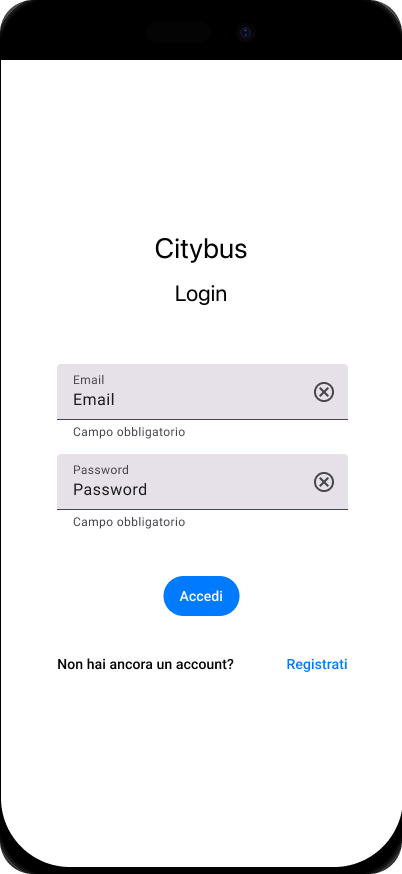
\includegraphics[width=\textwidth]{images/mockup/Login.png}
    \caption{Mockup Login - Versione Mobile}
    \label{fig:login-mobile}
  \end{minipage}
  \hfill
  \begin{minipage}[b]{0.68\textwidth}
    \centering
    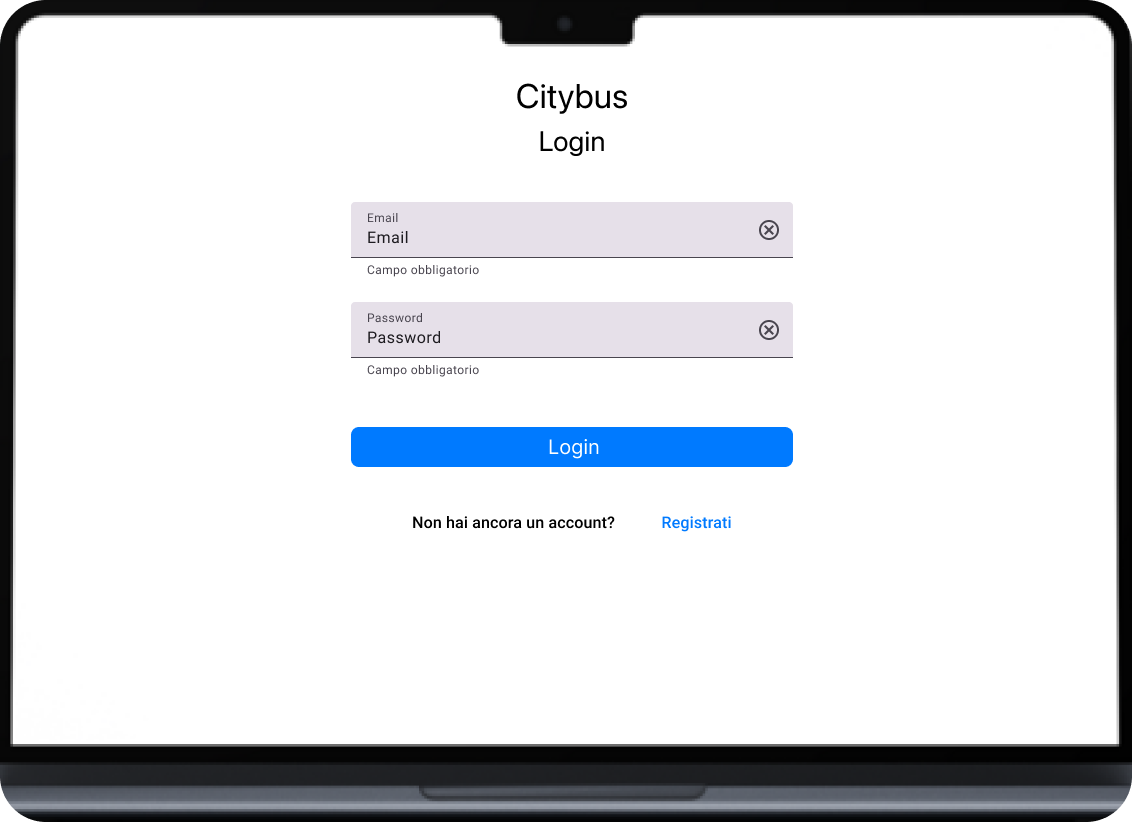
\includegraphics[width=\textwidth]{images/mockup/Login Desktop.png}
    \caption{Mockup Login - Versione Desktop}
    \label{fig:login-desktop}
  \end{minipage}
\end{figure}

Le due varianti di design si basano su un layout minimalista che evidenzia i campi di input (email e password), i messaggi di validazione, il pulsante di accesso e il link per la registrazione.

La pagina di registrazione costituisce il secondo step fondamentale nel flusso di autenticazione dell’applicazione Citybus, offrendo agli utenti un’interfaccia chiara per la creazione del proprio account. La disposizione dei campi (nome, cognome, email, password, conferma password) è pensata per guidare l’utente in un processo lineare e veloce, riducendo il rischio di errori e migliorando l’esperienza complessiva come si può vedere in Fig.\ref{fig:registrazione-mobile} e Fig.\ref{fig:registrazione-desktop}.

\begin{figure}[H]
  \centering
  \begin{minipage}[b]{0.25\textwidth}
    \centering
    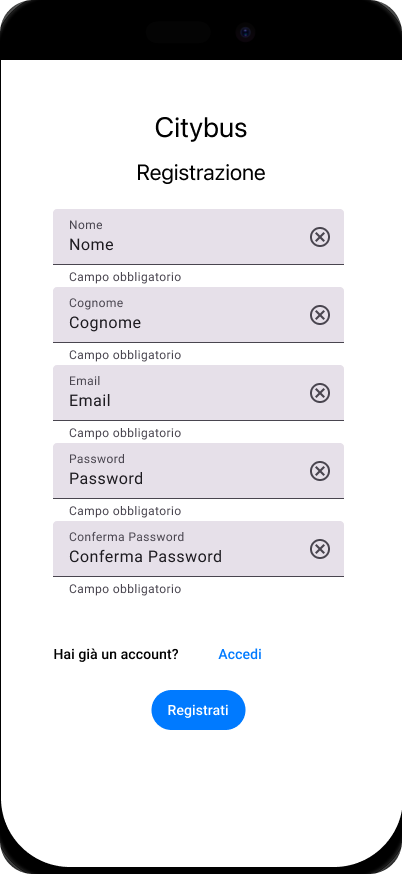
\includegraphics[width=\textwidth]{images/mockup/Registrazione.png}
    \caption{Mockup Registrazione - Versione Mobile}
    \label{fig:registrazione-mobile}
  \end{minipage}
  \hfill
  \begin{minipage}[b]{0.68\textwidth}
    \centering
    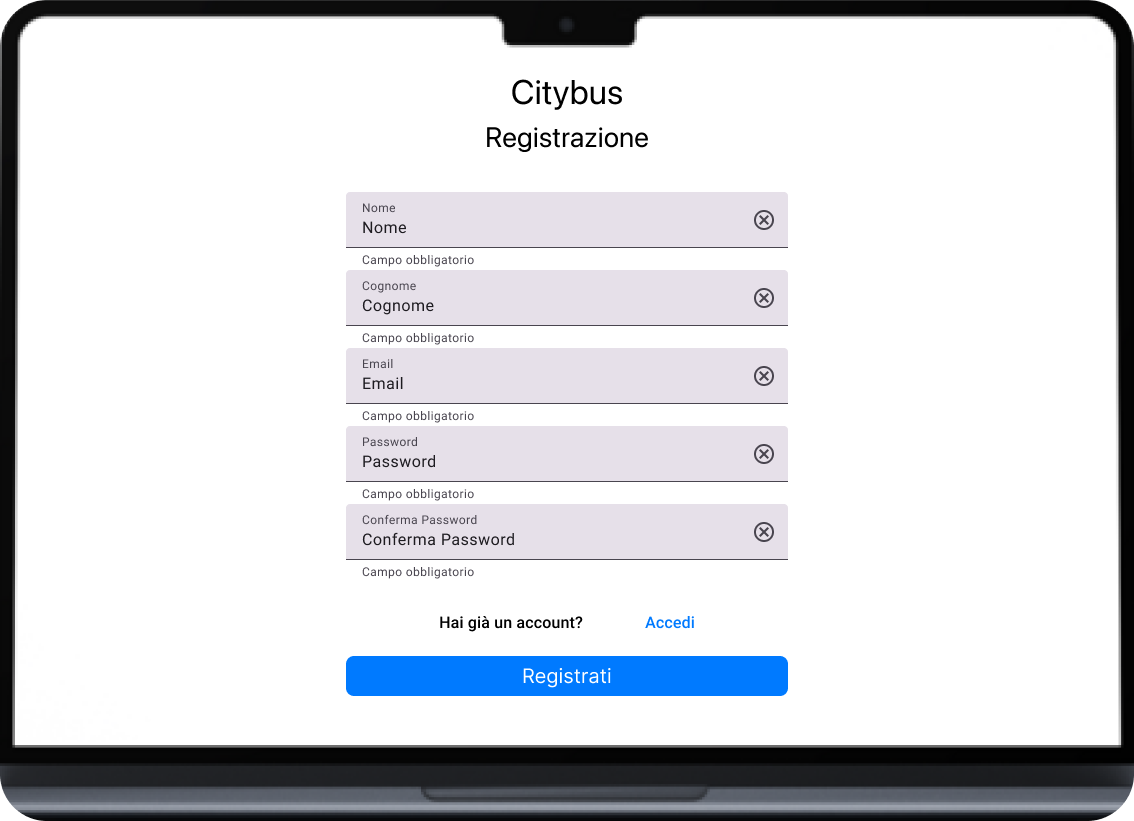
\includegraphics[width=\textwidth]{images/mockup/Registrazione Desktop.png}
    \caption{Mockup Registrazione - Versione Desktop}
    \label{fig:registrazione-desktop}
  \end{minipage}
\end{figure}

\subsubsection{Navigazione \& Partenze}

Una volta effettuata l'autenticazione si verrà portati alla pagina principale, ovvero alla pagina di navigazione, che si può vedere come il cuore dell'applicazione Citybus come mostrato in fig.\ref{fig:navigazione-cerca}, fig.\ref{fig:navigazione-percorso} e fig. \ref{fig:navigazione-desktop}.
La pagina permette all’utente di cercare e visualizzare il percorso più veloce per raggiungere la destinazione scelta utilizzando i mezzi pubblici. Il sistema consente di specificare il punto di partenza, la destinazione(queste ultime due inseribili tramite mappa o direttamente dai campi di input) e l’orario desiderato di partenza, per restituire in tempo reale la sequenza ottimale di fermate e la mappa interattiva con il percorso del bus.

\begin{figure}[H]
  \centering
  \begin{minipage}[b]{0.45\textwidth}
    \centering
    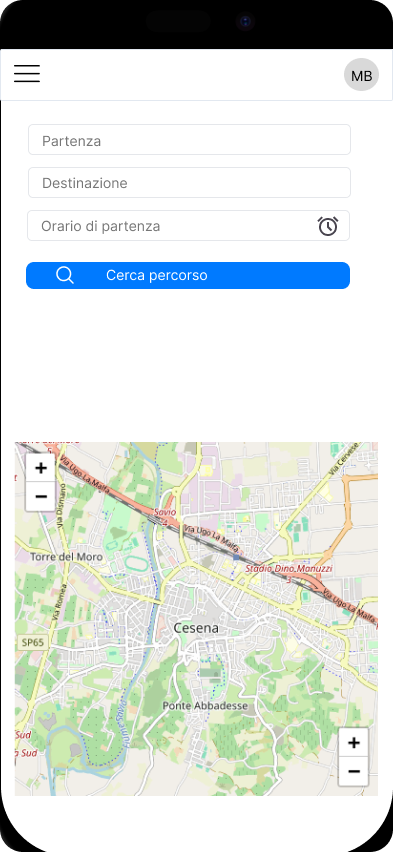
\includegraphics[width=\textwidth]{images/mockup/Cerca percorso.png}
    \caption{Navigazione Mobile - Ricerca percorso}
    \label{fig:navigazione-cerca}
  \end{minipage}
  \hfill
  \begin{minipage}[b]{0.45\textwidth}
    \centering
    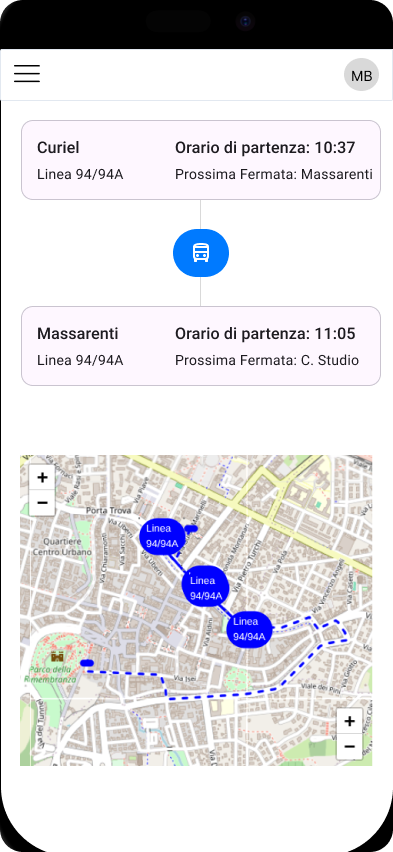
\includegraphics[width=\textwidth]{images/mockup/Percorso Trovato.png}
    \caption{Navigazione Mobile - Percorso trovato}
    \label{fig:navigazione-percorso}
  \end{minipage}
\end{figure}

\begin{figure}[H]
  \centering
  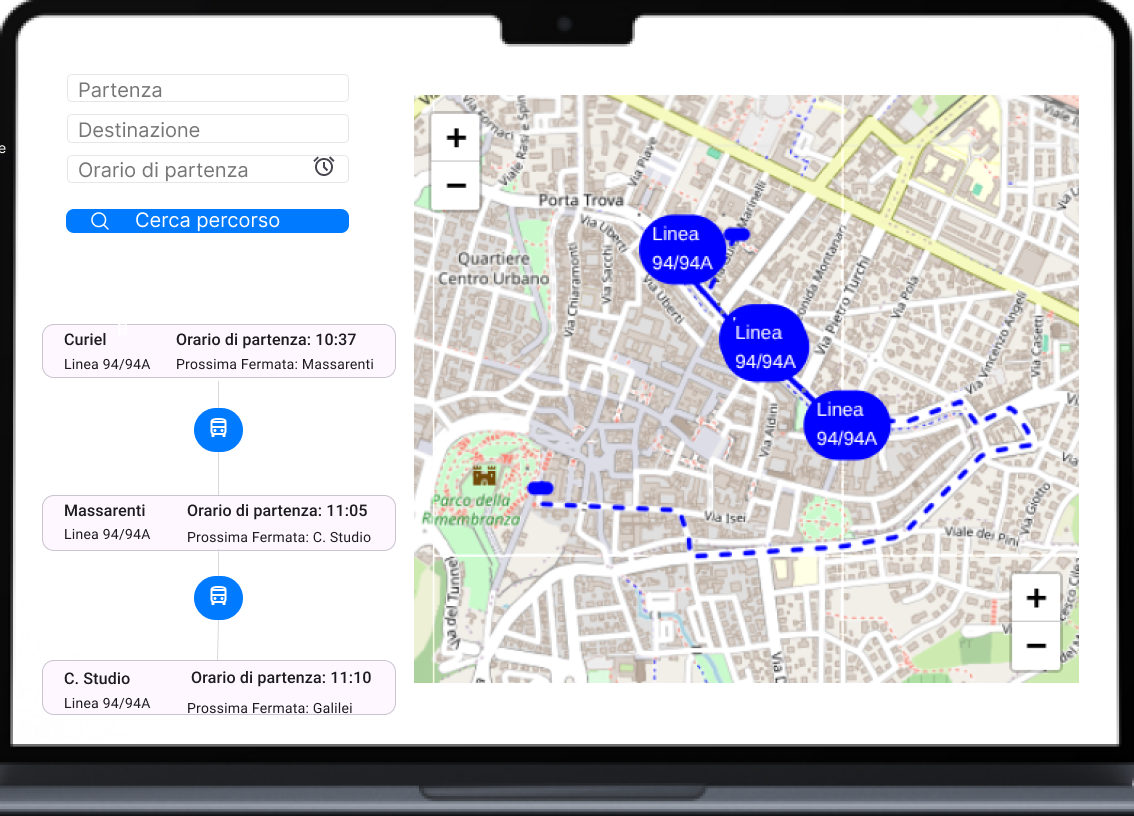
\includegraphics[width=\textwidth]{images/mockup/Navigazione Desktop.png}
  \caption{Navigazione - Versione Desktop}
  \label{fig:navigazione-desktop}
\end{figure}

La pagina delle partenze in fig.\ref{fig:partenze-desktop} completa il flusso principale dell’applicazione Citybus, offrendo agli utenti la possibilità di cercare le corse in arrivo presso una fermata specifica, a partire da un orario indicato. L’interfaccia è progettata per fornire un elenco chiaro delle corse previste, evidenziando lo stato di ciascuna di esse(in orario o in ritardo) e consentendo il monitoraggio dettagliato del percorso scelto.
Dalla vista mobile si prevede di interrompere il monitoraggio della linea grazie ad un apposito pulsante che permetta di tornare alla vista precedente come si può vedere in fig.\ref{fig:partenze-ricerca} e fig.\ref{fig:partenze-monitoraggio}.

\begin{figure}[H]
  \centering
  \begin{minipage}[b]{0.45\textwidth}
    \centering
    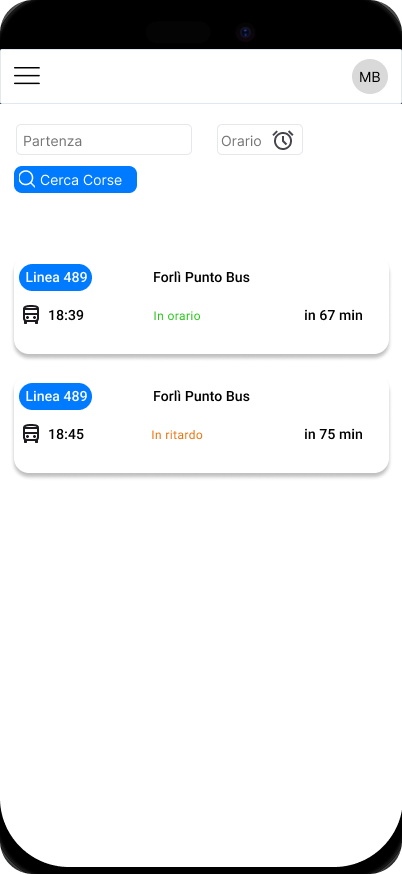
\includegraphics[width=\textwidth]{images/mockup/Ricerca Linee.png}
    \caption{Partenze - Mobile: Ricerca corse per fermata e orario}
    \label{fig:partenze-ricerca}
  \end{minipage}
  \hfill
  \begin{minipage}[b]{0.45\textwidth}
    \centering
    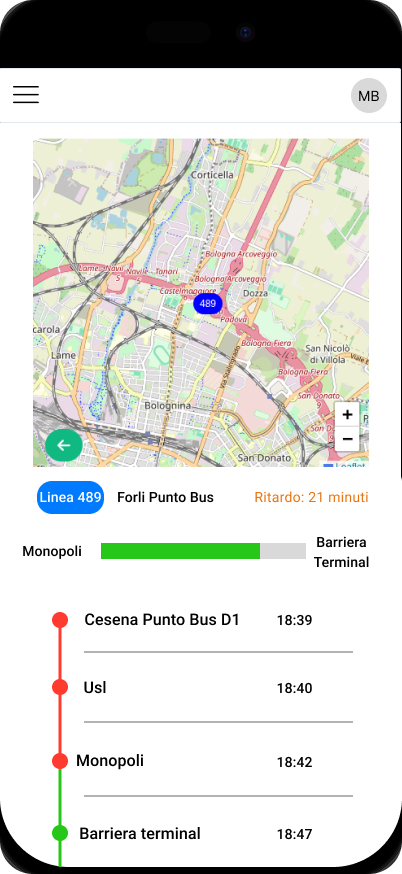
\includegraphics[width=\textwidth]{images/mockup/Monitoraggio linea.png}
    \caption{Partenze - Mobile: Monitoraggio corsa selezionata}
    \label{fig:partenze-monitoraggio}
  \end{minipage}
\end{figure}

\begin{figure}[H]
  \centering
  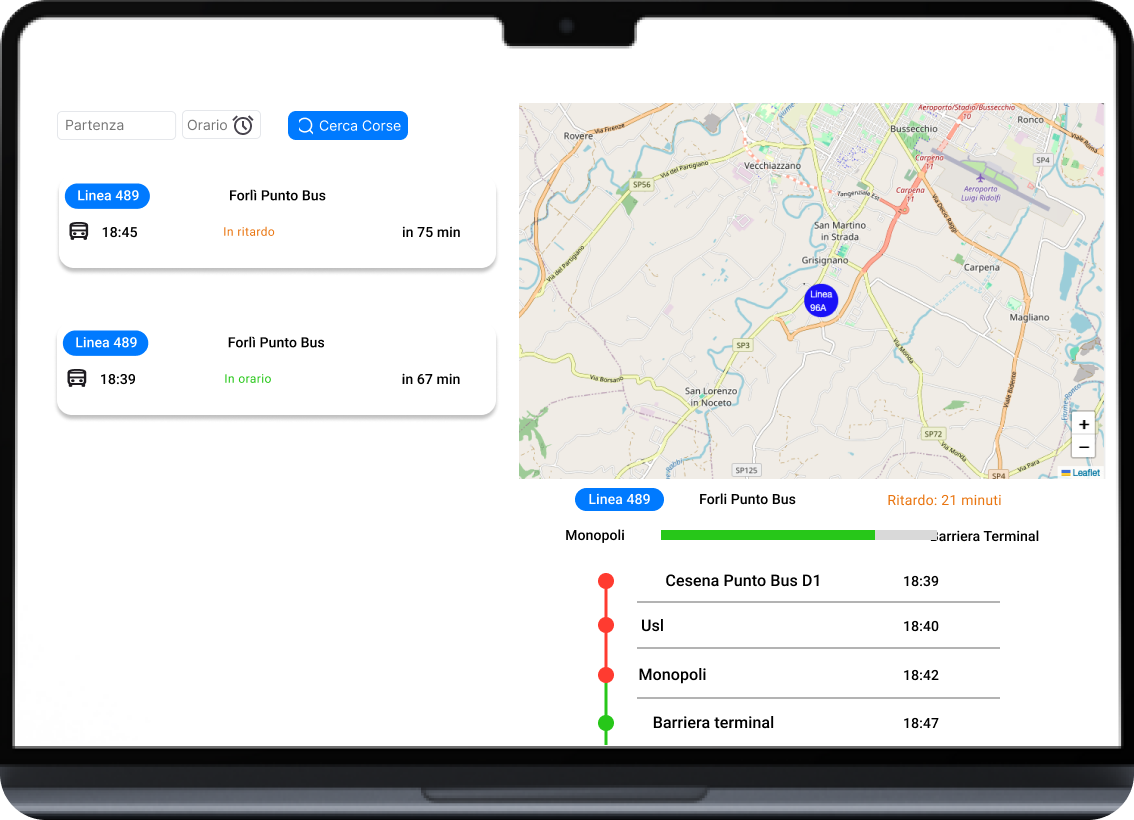
\includegraphics[width=\textwidth]{images/mockup/Ricerca Linee Desktop.png}
  \caption{Partenze - Versione Desktop: ricerca e monitoraggio corse}
  \label{fig:partenze-desktop}
\end{figure}

\subsubsection{Monitoraggio linee}

La pagina mostrata in fig.\ref{fig:monitoraggio_linee_desktop} e fig.\ref{fig:monitoraggio_linee_mobile}  è destinata agli amministratori dell’applicazione Citybus e fornisce una panoramica in tempo reale dello stato di tutte le corse attive sul territorio. Attraverso l’interfaccia, l’amministratore può monitorare ogni linea in servizio, filtrare le corse in ritardo e monitorare e seguire sulla mappa una corsa specifica una volta selezionata.
Questa interfaccia è progettata per supportare gli operatori nella gestione del servizio in tempo reale, garantendo un controllo completo sulla regolarità delle corse e facilitando interventi rapidi in caso di criticità.

\begin{figure}[H]
  \centering
  \begin{minipage}[b]{0.25\textwidth}
    \centering
    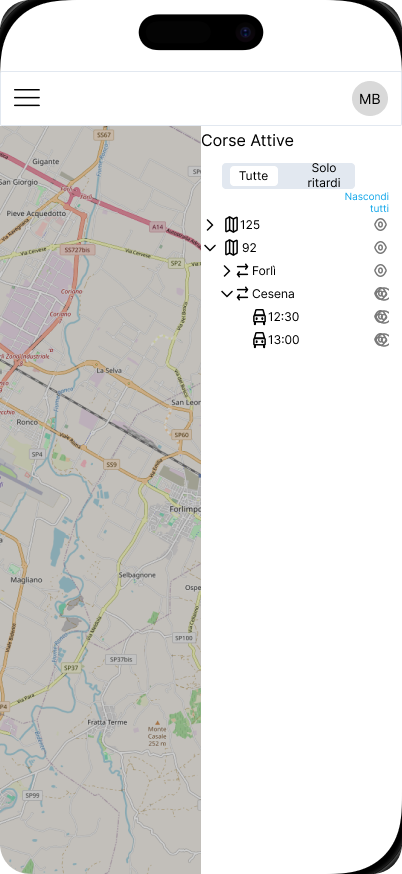
\includegraphics[width=\textwidth]{images/mockup/Mappa Linee.png}
    \caption{Monitoraggio linee - Desktop}
    \label{fig:monitoraggio_linee_desktop}
  \end{minipage}
  \hfill
  \begin{minipage}[b]{0.68\textwidth}
    \centering
    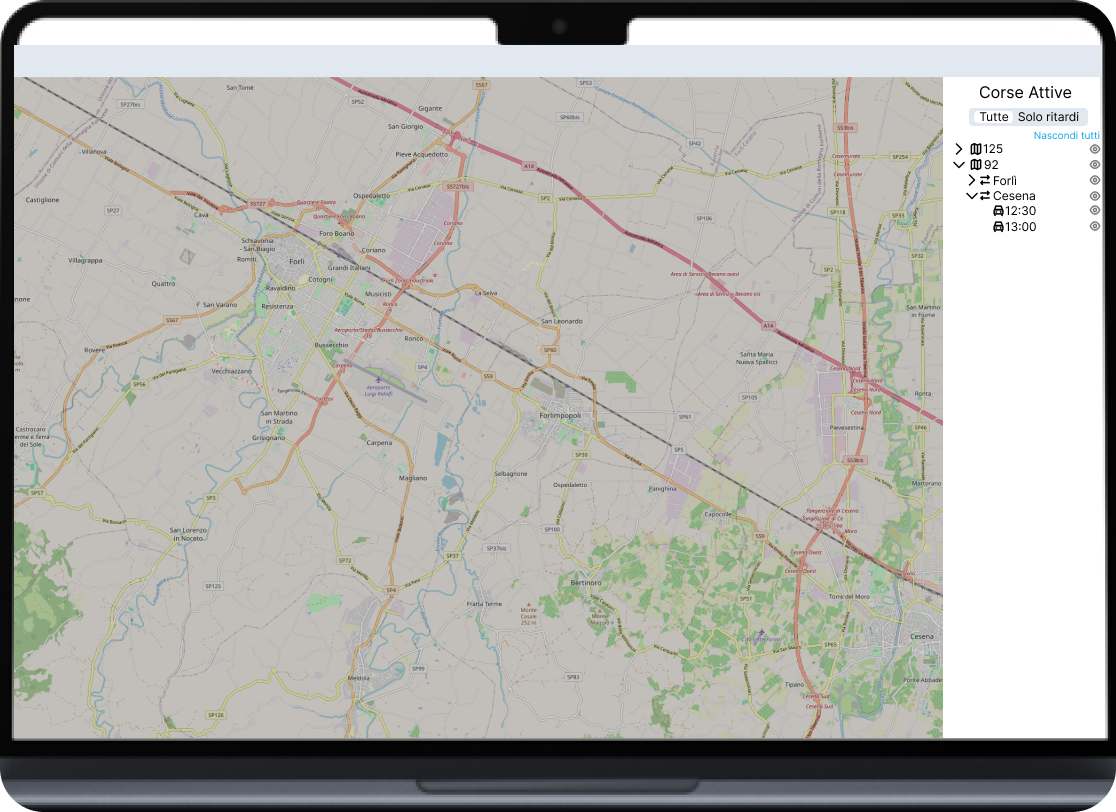
\includegraphics[width=\textwidth]{images/mockup/Mappa.png}
    \caption{Monitoraggio linee - Mobile}
    \label{fig:monitoraggio_linee_mobile}
  \end{minipage}
\end{figure}

\subsubsection{Creazione linee}

Il processo di creazione di una nuova linea è stato suddiviso in 3 step in modo da rendere il tutto più intuitivo e ordinato.
Il primo step permette di inserire le informazioni di base necessarie per la configurazione del servizio. Gli utenti amministratori possono definire:
\begin{itemize}
    \item il nome della linea
    \item le diverse direzioni associate alla linea, aggiungendo o rimuovendo voci in modo dinamico.
\end{itemize}
Le figure \ref{fig:nuova-linea-desktop-step1} e \ref{fig:nuova-linea-mobile-step-1} mostrano questo primo step.

\begin{figure}[H]
  \centering
  \begin{minipage}[b]{0.25\textwidth}
    \centering
    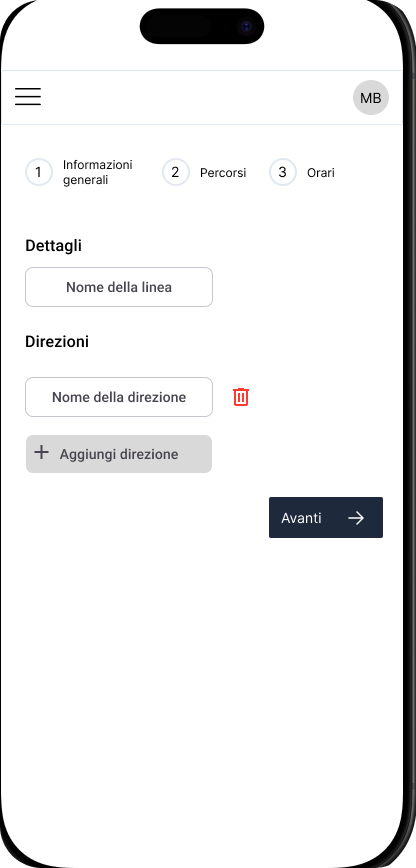
\includegraphics[width=\textwidth]{images/mockup/Nuova Linea Step 1.png}
    \caption{Creazione Nuova Linea - Mobile: Inserimento informazioni generali}
    \label{fig:nuova-linea-mobile-step-1}
  \end{minipage}
  \hfill
  \begin{minipage}[b]{0.68\textwidth}
    \centering
    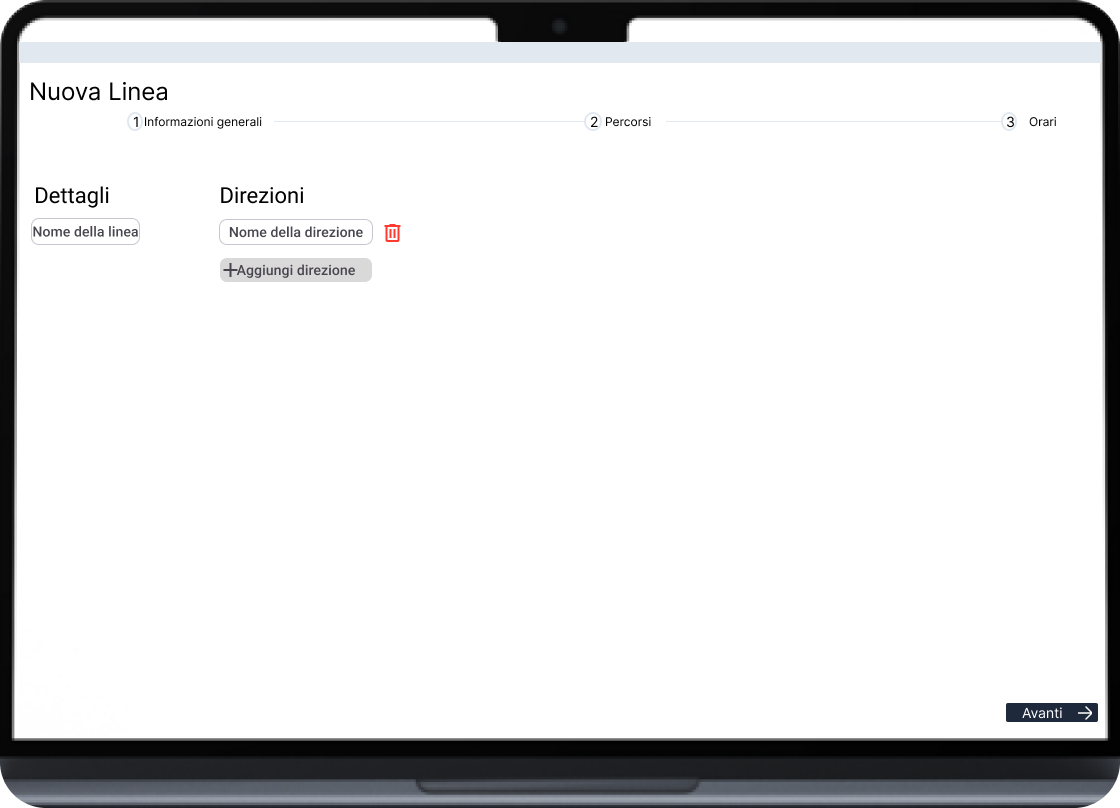
\includegraphics[width=\textwidth]{images/mockup/Nuova-Step1_desktop.png}
    \caption{Creazione Nuova Linea - Desktop: Inserimento informazioni generali}
    \label{fig:nuova-linea-desktop-step1}
  \end{minipage}
\end{figure}

Nel secondo step della procedura guidata mostrata in fig.\ref{fig:nuova-linea-step2-mobile} e fig.\ref{fig:nuova-linea-step2-desktop} per la creazione di una nuova linea, l’utente definisce il percorso dettagliato per ogni direzione configurata in precedenza. In questa schermata è possibile:

\begin{itemize}
    \item inserire le fermate attraverso un elenco ordinato, scegliendo fermate già esistenti o aggiungendole direttamente dalla mappa
    \item visualizzare i tempi di percorrenza stimati tra le fermate, aggiornati dinamicamente
    \item generare automaticamente il percorso sulla mappa tramite il pulsante “Genera percorso”, che calcola il tragitto più efficiente in base all’ordine delle fermate
\end{itemize}

La mappa interattiva mostra immediatamente la traiettoria generata, permettendo un riscontro visivo istantaneo sul percorso configurato. La suddivisione in tab per ogni direzione (es. Direzione 1, Direzione 2, Direzione 3) rende l’esperienza semplice e ordinata anche per linee complesse con più direzioni.

\begin{figure}[H]
  \centering
  \begin{minipage}[b]{0.25\textwidth}
    \centering
    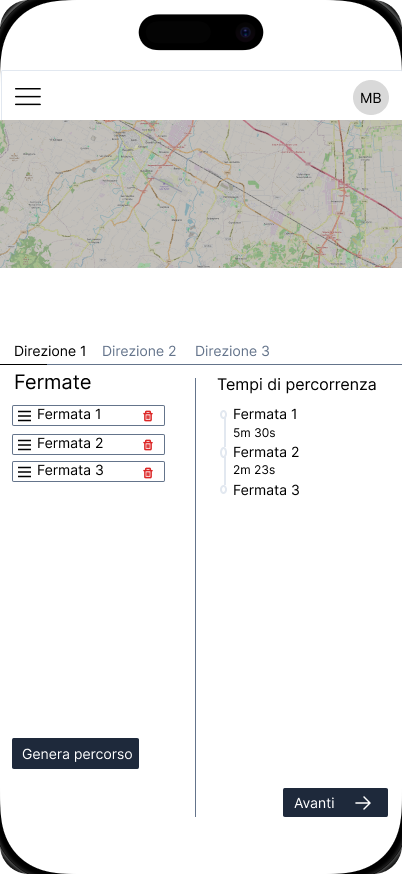
\includegraphics[width=\textwidth]{images/mockup/Creazione linea Step 2.png}
    \caption{Creazione Nuova Linea - Mobile: Inserimento fermate e generazione percorso}
    \label{fig:nuova-linea-step2-mobile}
  \end{minipage}
  \hfill
  \begin{minipage}[b]{0.68\textwidth}
    \centering
    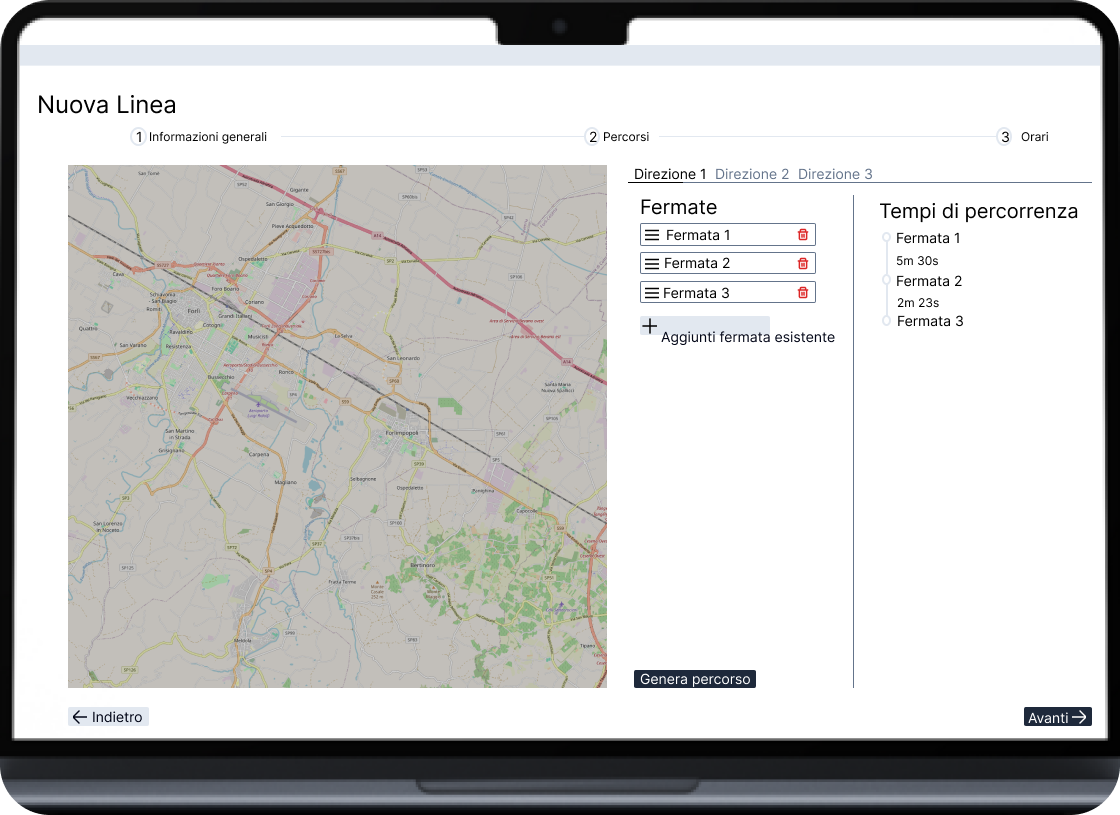
\includegraphics[width=\textwidth]{images/mockup/Nuova Linea Step 2.png}
    \caption{Creazione Nuova Linea - Desktop: Inserimento fermate e mappa percorso}
    \label{fig:nuova-linea-step2-desktop}
  \end{minipage}
\end{figure}

Come si può vedere nelle fig.\ref{fig:nuova-linea-step3-mobile} e \ref{fig:nuova-linea-step3-desktop}, il terzo e ultimo step della procedura guidata per la creazione di una nuova linea consente all’amministratore di configurare gli orari di partenza per ciascuna direzione definita. Inserendo un orario di partenza, il sistema calcola automaticamente gli orari stimati di arrivo per tutte le fermate della direzione, sulla base dei tempi di percorrenza impostati nello step precedente.

\begin{figure}[H]
  \centering
  \begin{minipage}[b]{0.25\textwidth}
    \centering
    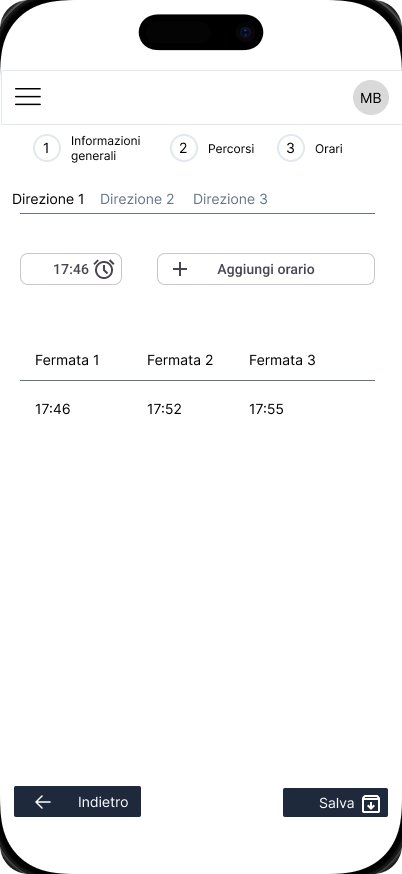
\includegraphics[width=\textwidth]{images/mockup/Creazione linea Step 3.png}
    \caption{Creazione Nuova Linea - Mobile: Inserimento orari di partenza e arrivo alle fermate}
    \label{fig:nuova-linea-step3-mobile}
  \end{minipage}
  \hfill
  \begin{minipage}[b]{0.68\textwidth}
    \centering
    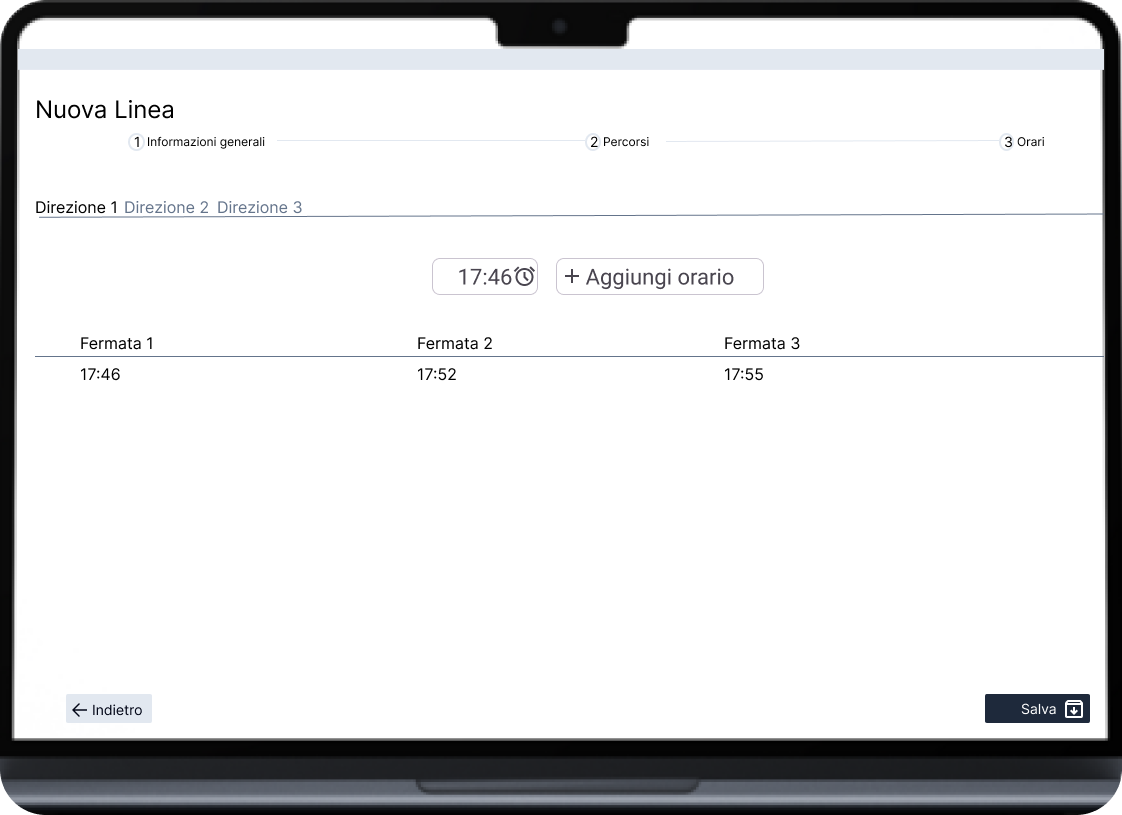
\includegraphics[width=\textwidth]{images/mockup/Nuova Linea Step 3 Desktop.png}
    \caption{Creazione Nuova Linea - Desktop: inserimento orari e visualizzazione arrivi}
    \label{fig:nuova-linea-step3-desktop}
  \end{minipage}
\end{figure}

\subsubsection{Gestione linee}

La pagina di gestione delle linee rappresenta il centro di controllo per gli amministratori, permettendo la supervisione completa di tutte le linee configurate nell’applicazione. Attraverso una tabella chiara e ordinata, è possibile:
\begin{itemize}
    \item visualizzare in un colpo d’occhio tutte le linee con le relative direzioni, partenze e arrivi.
    \item selezionare una o più linee per effettuare azioni di modifica o eliminazione.
    \item Avviare la procedura di creazione di una nuova linea tramite il pulsante “Nuova Linea”.
\end{itemize}

Questa schermata, disponibile nelle versioni mobile(fig.\ref{fig:gestione-linee-mobile} e desktop(fig.\ref{fig:gestione-linee-desktop}, è progettata per semplificare al massimo la gestione della rete di trasporto

\begin{figure}[H]
  \centering
  \begin{minipage}[b]{0.25\textwidth}
    \centering
    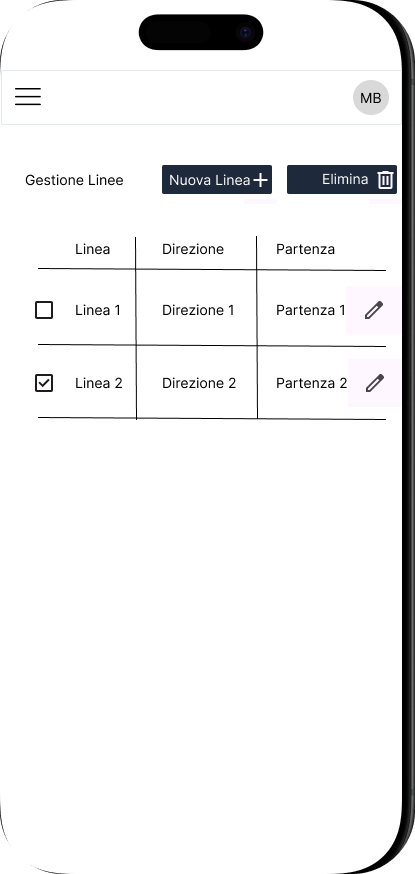
\includegraphics[width=\textwidth]{images/mockup/Gestione Linee Mobile.png}
    \caption{Gestione Linee - Mobile: tabella linee con azioni di modifica ed eliminazione}
    \label{fig:gestione-linee-mobile}
  \end{minipage}
  \hfill
  \begin{minipage}[b]{0.68\textwidth}
    \centering
    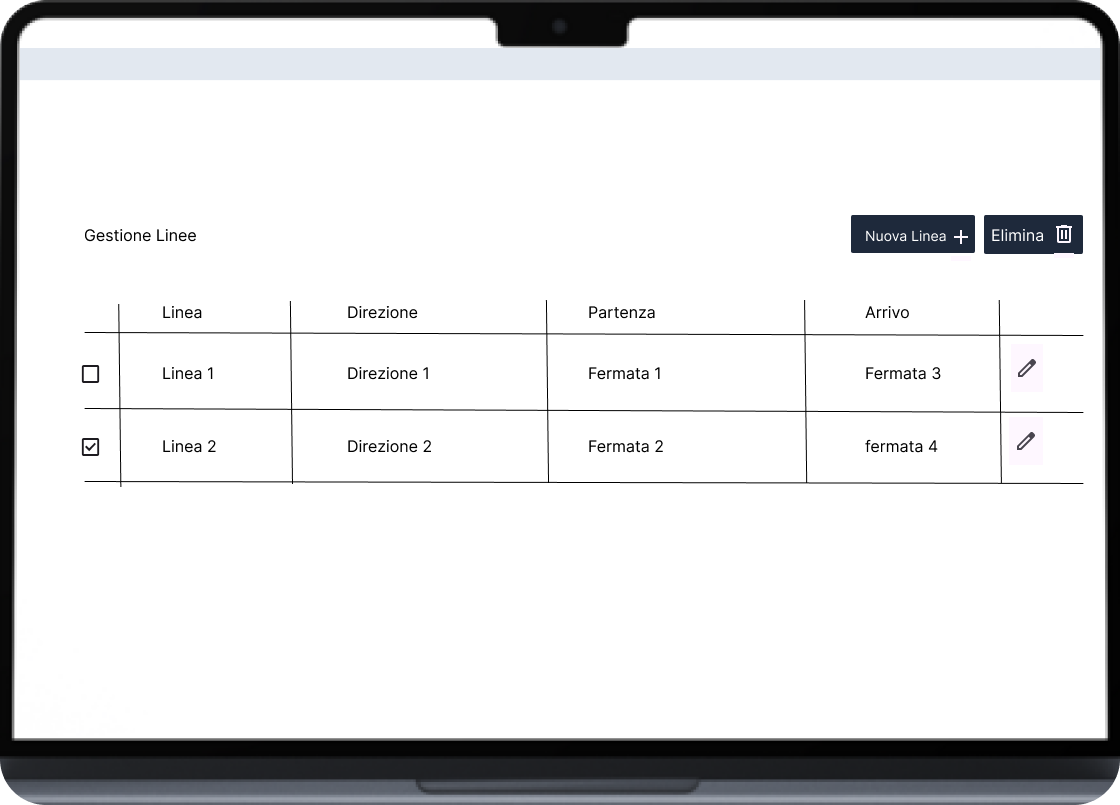
\includegraphics[width=\textwidth]{images/mockup/Gestione Linee Desktop.png}
    \caption{Gestione Linee - Desktop: panoramica linee e funzionalità di amministrazione}
    \label{fig:gestione-linee-desktop}
  \end{minipage}
\end{figure}
